\documentclass{article}
\usepackage{graphicx} % Required for inserting images
\usepackage{subcaption}
\usepackage{amsmath}
\title{Documentation Up To 8 April}
\author{Carles Roca Reverter}
\date{April 2024}

\begin{document}

\maketitle

\section{Introduction}

1.\\
After reading the corresponding papers to understand the problem formulation and current state-of-art() and the proposed algorithm to solve the optimization (MVRSM, surrogate model) we tested some single-objective and multi-objective functions on the algorithm to how to format our future function and to check that it works correctly.\\
For instance, trying with the multi-objective (2 objectives) Binh and Korn function we get this correct convex Pareto Set.
\begin{figure}[h] %Recorda fixar la posició de les figures si no
	\centering
	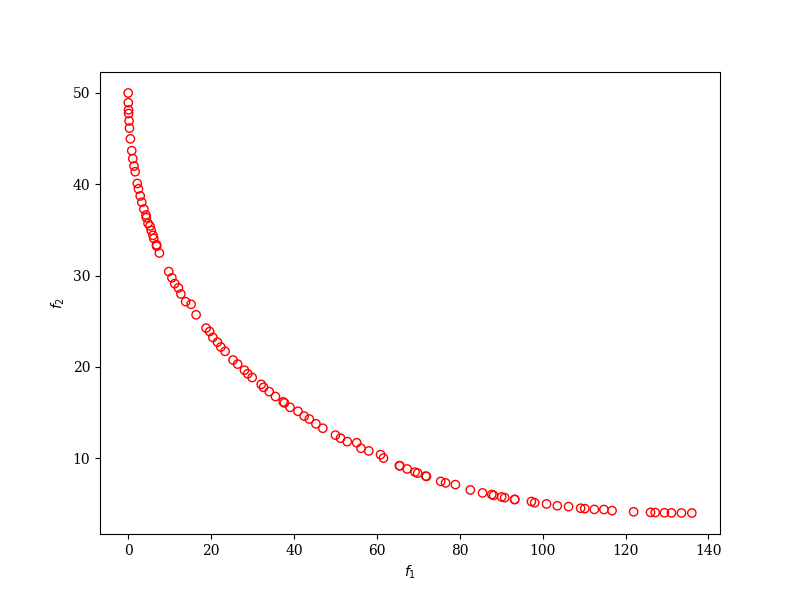
\includegraphics[width=1.1\textwidth]{imatges/binhorn_propi.png}
	\caption{Convex Pareto Set obtained for Binh and Korn function with MVRSM multi-objective}
	\label{fig:binhkorn} %Si es posen les etiquetes de forma ordenada, la vida es més fàcil...
\end{figure}\\

2.  After that, we studied the grid to be analysed and defined the admittance matrix in terms of their parameters and the cost function function to evaluate when using HVAC.\\
Note that in the power flow all buses are considered PQ buses excpet bus 6, which is the slack bus and represents the grid we are supplying power to. Also, we are allowing the reactive power compensation to be placed in the 5 different posible positions trough the line (pre and post offshore trafo, midcable and pre and post onshore trafo), rather than just 3

%\section{Objective function AC
%}
%\begin{gather*}
%F_{obj}(x)=C_{cb-AC}+C_{gis-AC}+C_{tr}+C_{ss-AC}+C_{loss-%AC}+C_{react}=\\\\ \frac{(A+Be^{CS_{r-cb}}+D)\cdot(9n+1)}{10E}\cdot l +
%0.0117\cdot U_{AC-N}+0.0231+0.0427\cdot S_{r-tr}^{0.7531}+2.534+ \\\\+0.0887\cdot P_{owf-N}+8760\cdot t_{owf}\cdot C_E\cdot\sum_{j=1}^{N_w}(P_{loss-j}\cdot p_{w-j)}+ \sum_{i=1}^{N_{react}}(Y_{l-i}^{max}\cdot K + P)
%\end{gather*}\\
%\[P_{loss-AC}=(p_{owf}-p_g)S_b=(p_{owf}-Re\{\underline{s}_5\})S_b\]

\section{Vector of unknowns
}

\begin{itemize}
  \item Binary variables of the shunt reactors: Binary. Whether we put or not a shunt reactor at position i. 
  \item Transmission voltage: Choice ( a integer number is assigned which corresponds to a set of parameters for that voltage level)
  \item Number of cables: Integer
  \item Transformer rated power: Continuous
  \item Shunt reactors value: Continuous. Sizing of the compensation at position i.
\end{itemize}
\section{Constraints AC}
Equality constraints: POWER FLOW
\\
\[\mathbf{h_m(x)=0}\]
\[\mathbf{S_i=V_i(\sum_{j=1}^{N_{nodes}}Y_{ij}V_j)^*}\]
\[\underline{s}_1-(p_{owf}+jq_{owf})=0\]
\[\underline{s}_1-\underline{u}_1[(2\underline{y}_{tr}+\underline{y}_l)\underline{u}_1-(\underline{y}_{tr})\underline{u}_2]^*=0\]
\[\underline{s}_2-\underline{u}_2[-(\underline{y}_{tr})\underline{u}_1+(2\underline{y}_{\pi1}+\underline{y}_l+\underline{y}_{tr})\underline{u}_2-(\underline{y}_{\pi1})\underline{u}_3]^*=0\]
 \[\underline{s}_3-\underline{u}_3[-(\underline{y}_{\pi1})\underline{u}_2+(2\underline{y}_{\pi1}+2\underline{y}_{\pi2}+\underline{y}_{l})\underline{u}_3-(\underline{y}_{\pi2})\underline{u}_4]^*=0\]
 \[\underline{s}_4-\underline{u}_4[-(\underline{y}_{\pi2})\underline{u}_3+(2\underline{y}_{\pi2}+\underline{y}_l+\underline{y}_{tr})\underline{u}_4-(\underline{y}_{tr})\underline{u}_5]^*=0\]
 \[\underline{s}_5-\underline{u}_5[-(\underline{y}_{tr})\underline{u}_4+(2\underline{y}_{tr}+\underline{y}_l+\underline{y}_{g})\underline{u}_5]^*=0\]\\\\
 \[\mathbf{Y}=\begin{bmatrix}
 (2\underline{y}_{tr}+\underline{y}_l) & -\underline{y}_{tr} & 0 & 0 & 0 & 0\\
-\underline{y}_{tr} & (2\underline{y}_{\pi1}+\underline{y}_l+\underline{y}_{tr}) & -\underline{y}_{\pi1} & 0 & 0 & 0  \\
0 & -\underline{y}_{\pi1} & (2\underline{y}_{\pi1}+2\underline{y}_{\pi2}+\underline{y}_{l}) & -\underline{y}_{\pi2}   & 0 & 0 \\
0 & 0 & -\underline{y}_{\pi2} & (2\underline{y}_{\pi2}+\underline{y}_l+\underline{y}_{tr}) & -\underline{y}_{tr} & 0  \\
0 & 0 & 0 & -\underline{y}_{tr} & (2\underline{y}_{tr}+\underline{y}_l+\underline{y}_{g}) & -\underline{y}_{g}  \\
0 & 0 & 0 & 0 & -\underline{y}_{g} & \underline{y}_{g}\\
\end{bmatrix}\] \\



%%\[s_1-(p_{owf}+jq_{owf})=0\]
%%\[s_1-u_1[(y_{tr}+y_l)u_1+i_2]^*=0\]
%\[u_2-(u_3+z_{\pi1}i_3)=0\]
%\[s_2-u_2[(y_{\pi1}+y_l)u_2+i_3]^*=0\]
%\[s_3-u_3[(y_{\pi1}+y_l+y_{\pi2})u_3+i_4]^*=0\]
%\[u_3-(u_4+z_{\pi2}i_4)=0\]
%%\[u_4-(u_5+z_{tr}i_5)=0\]
%\[s_5-u_5[(y_{tr}+y_l)u_5+i_g]^*=0\]
%\[u_5-(u_g+z_{g}i_g)=0\]

Inequality constraints: LIMITATIONS
\\
\[\mathbf{g_n(x)\leq0}\]
\[U_{kj}-U_{max}\leq0\]
\[U_{min}-U_{kj}\leq0\]
\[I_{kj}-I_{max}\leq0\]
\[Q_{min}-Q_{gj}\leq0\]
\[Q_{gj}-Q_{max}\leq0\]
\[Y_{l-ij}-Y_{l-i}^{max}\leq0\]
\[N_{react}-N_{react}^{max}\leq0\]

\newpage
\section{Newton-Rapshon Solver code
}
For solving the PF, we code a simple solver using the Newton-Rapshon method. Note we are computing the Jacobian with the explicit form (derivatives) rather than numerically, which yields faster results.\\
After solving the PF, we compute technical costs with their corresponding penalization and the investment resulting from the decided combination of parameters.\\
A fist trial was intended using single-objective, which means you sum up all the costs as objective and try to minimize that using MRVSM. We obtained the following results:
\begin{figure}[h] %Recorda fixar la posició de les figures si no
    \centering
	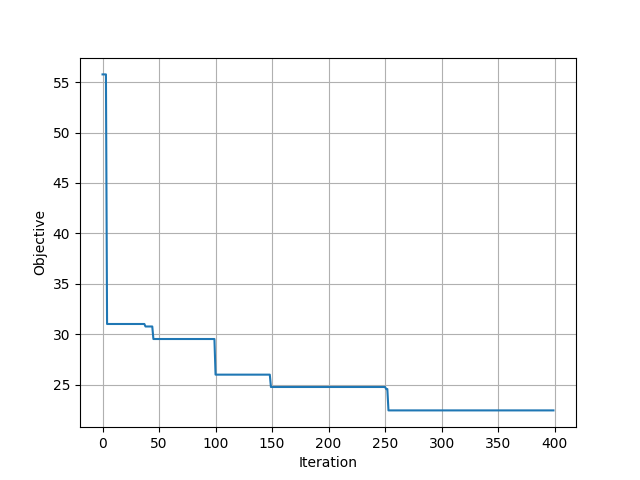
\includegraphics[width=0.6\textwidth]{imatges/evolucio_iter.png}
	\caption{Evolution of cost function objective as iterations go on}
	\label{fig:binhkorn} %Si es posen les etiquetes de forma ordenada, la vida es més fàcil...
\end{figure}\\

As we can see, it seems the algorithm is able to minimize the objective function and follows a reasonable path. Nevertheless it would be interesting to start evaluating the problem as a multi-objective. Why? This way we can evaluate the trade off between investments and technical costs and therefore try to find the Pareto set of our optimization problem.\\
\subsection{Multi-objective}
Then, we adaptades the cost function for a multi-objective output and uses the correspondent form of the MVRSM. As a first step we consider a fixed value for transmission voltage and number of cables, without adding any reactor and let free the trafo powers variable to see if the problem definitions is well formulated. As we can see in the image we have 2 good news: We are getting the set of points we were expecting and the algorithm is converging to the optimal ones (see how the color of the points indicates the evolution). Yellow points from the last iterations are falling in the optimal zones.
\newpage
\begin{figure}[h] %Recorda fixar la posició de les figures si no
    \centering
	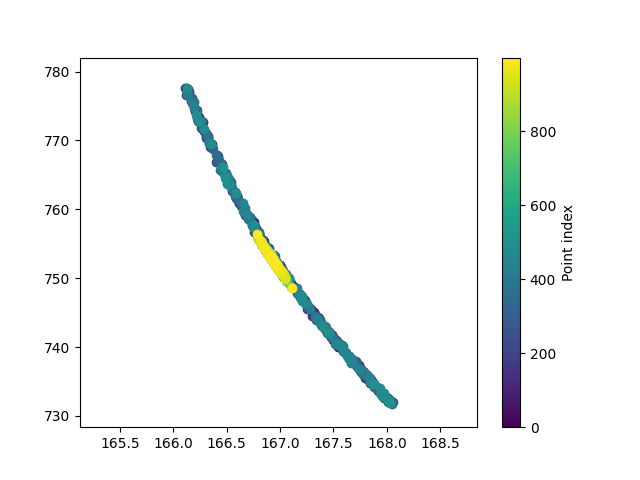
\includegraphics[width=0.8\textwidth]{imatges/costos_reacnoestanbe.png}
	\caption{Convex Pareto Set letting only trafo rated power as free variable (x-axis is investment, y-axis is tech cost)}
	\label{fig:binhkorn} %Si es posen les etiquetes de forma ordenada, la vida es més fàcil...
\end{figure}
Now it is interesting to add the compensations as potential investment and also let transmission voltage and number of cables as free parameters. If we let the function to introduce just one compensator (for instance an offshore one between the plant and the trafo) we obtain the following:
\begin{figure}[h] %Recorda fixar la posició de les figures si no
    \centering
	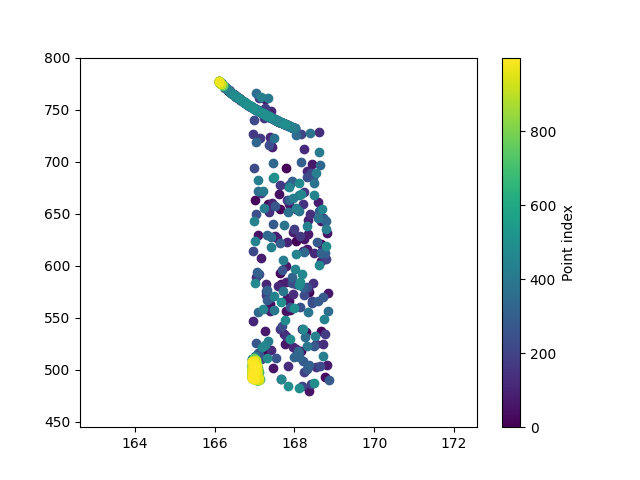
\includegraphics[width=0.51\textwidth]{imatges/1react.png}
	\caption{Plot fix vol and just 1 reactor}
	\label{fig:binhkorn} %Si es posen les etiquetes de forma ordenada, la vida es més fàcil...
\end{figure}
Clearly the top curved part corresponds to the combinations where it is NOT adding the shunt reactance and the only free parameter is the trafo (same result as before). Is difficult for me to interpret this results, since it seems like the cost of adding is so small compared to other ones. If we virtually (multiplying by a factor x10) increase the reactors costs and allow for all possible combinations:
\newpage
\begin{figure}[h] %Recorda fixar la posició de les figures si no
    \centering
	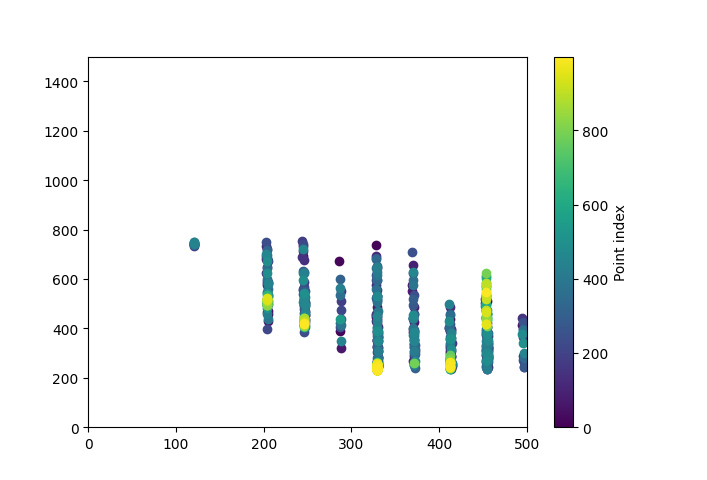
\includegraphics[width=0.8\textwidth]{imatges/pareto_discret.png}
	\caption{Discrete combinations of reactors}
	\label{fig:binhkorn} %Si es posen les etiquetes de forma ordenada, la vida es més fàcil...
\end{figure}
Here we kind of see a "discretized" Pareto of the reactor combinations. Note here we can see the first signs of Lauren's comments about the difficulty of convergence of the algorithm for non-convex and smooth Pareto's, as it seems that the final iterations are not always leading to optimal points.\\

Now we want to put all variables into play, including different voltages levels and number of cables. 
\begin{figure}[h] %Recorda fixar la posició de les figures si no
    \centering
	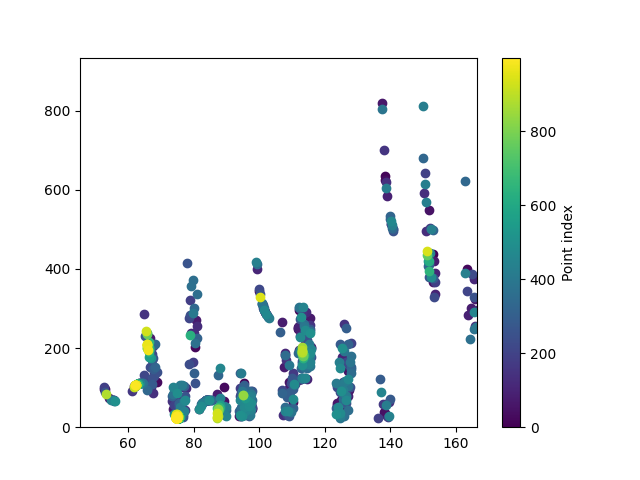
\includegraphics[width=0.6\textwidth]{imatges/react1i2.png}
	\caption{Reactors 1 and 2 and all combinations of voltages and number of cables}
	\label{fig:binhkorn} %Si es posen les etiquetes de forma ordenada, la vida es més fàcil...
\end{figure}
\newpage
We can also plot the Pareto dominant points:
\begin{figure}[h] %Recorda fixar la posició de les figures si no
    \centering
	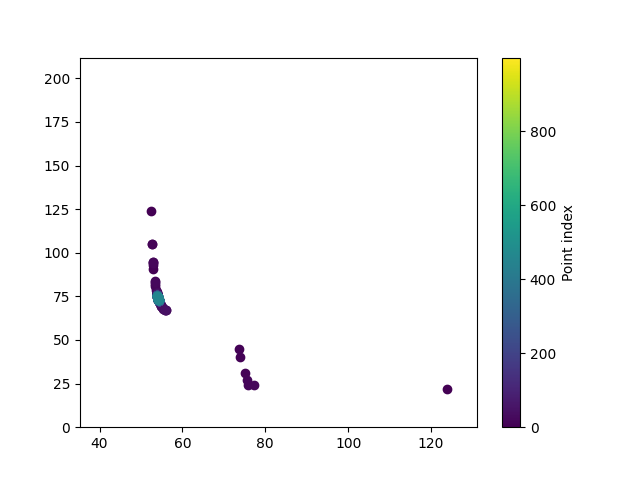
\includegraphics[width=0.6\textwidth]{imatges/paretofront.png}
	\caption{Pareto set: note it is a zoom to the lower left part of previous plot}
	\label{fig:binhkorn} %Si es posen les etiquetes de forma ordenada, la vida es més fàcil...
\end{figure}
To see how useful is the algorithm, wee can compare the results obtained with a random search of 1000 evaluations (now all 5 reactors are considered).
\begin{figure}[h] %Recorda fixar la posició de les figures si no
    \centering
	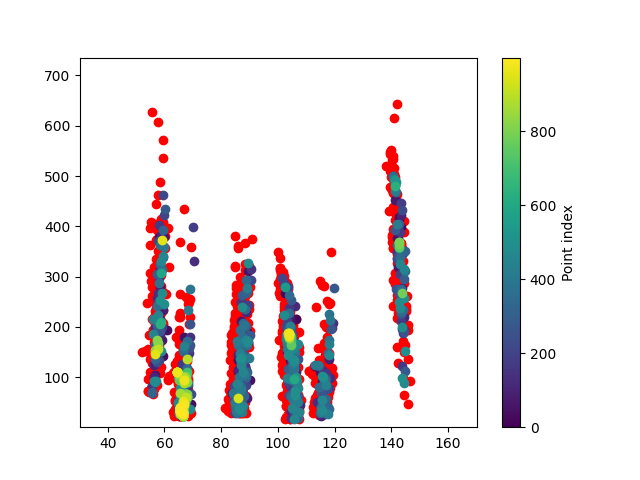
\includegraphics[width=0.6\textwidth]{imatges/superposat.png}
	\caption{Red dots are purely random evaluations}
	\label{fig:random} %Si es posen les etiquetes de forma ordenada, la vida es més fàcil...
\end{figure}
From this random evaluation we can infer the following. For the current definition of the problem the algorithm is not being that useful because a relatively small set of random evaluation s is able to "reach" the optimal solutions too. This could be due by the fact that only a small number of possible investments is considered and computationally talking it es easy to reach optimal operating points by just "brute force" using random evaluations.\\
Also we can try to somehow simulate what would happen if we used the  voltage variable as a continuous range, which is not feasible in reality, to check if somehow we can obtain a smoother plot and indicate that we are in the right direction. Note that to do that we have to "invent" a cost function (which is in reality of discrete nature and does not follow a clear continuous function). That's why the order of magnitude of the following results must not be taken as representative, but just as an experiment trying to simulate this extra continuous variable.
\begin{figure}[h] %Recorda fixar la posició de les figures si no
    \centering
	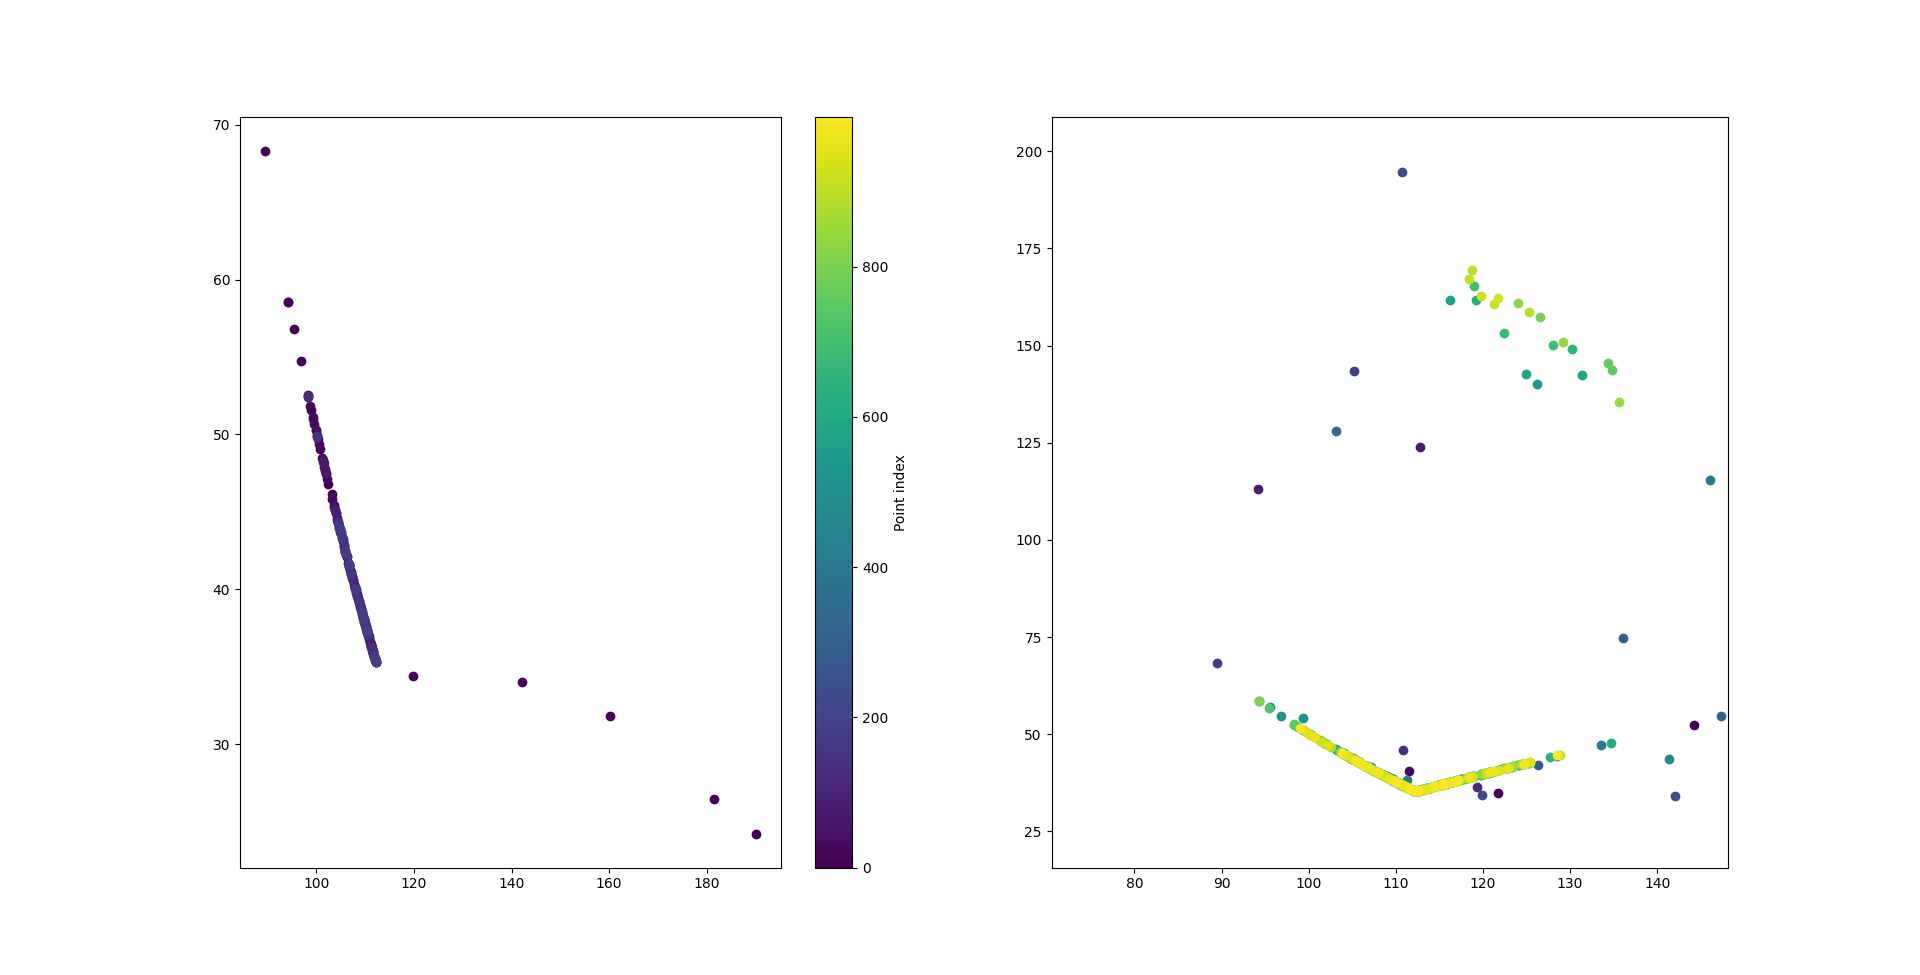
\includegraphics[width=1.2\textwidth]{imatges/pareto_volcontinu.png}
	\caption{Dominant points (left) and obtained points (right) with continuous transmission voltage level.}
	\label{fig:random} %Si es posen les etiquetes de forma ordenada, la vida es més fàcil...
\end{figure}

\section{Next steps
}
Next steps are the following one:
\begin{itemize}
  \item Try to modify MVRSM for non-convex Pareto sets using the tricks commented by Laurens. Fixating at the worst objective at each iteration.
  \item Study if there are more useful algorithms for this king of problem such as genetic ones (i.e. NSGA-II or NSGA-III) .
  \item Ponder different wind conditions in the cost calculation using probability to take into account different power generations and needs of reactive compensation.
  \item Go for a further complex analysis which considers the meshing between the turbines inside the wind power plant (electrical collection system). This includes a much bigger number of decision variables in the problem (discrete) , which potentially would allow to really take advantage of MVRSM strength and derive into a smoother Pareto set.
\end{itemize}


\section{NSGA-II
}
Now we will expose the first results obtained when implementing a new type of algorithm: NSGA-II with uses a meta-heuristic genetic approach.\\
general first impressions:
\begin{itemize}
  \item Results are better than MVRSM
  \item Each voltage level and/or number of cables has to be evaluated separately (to avoid power flow not converging in any of them) to get good results. If not, algorithm "breaks" when the PF dos not converge.
  \item For now, technical constraints are treated with a penalty function. To determine optimal point in the pareto set, since weights and importance are not fully clear, I would go for an utopia point analysis with the Pareto front.
  \item We should investigate how the different crowding functions work and which suits better (seems we get similar results with all the 2-objective oriented ones)

\end{itemize}
We attach some results obtained:
\begin{figure}[h]
  \begin{subfigure}{\linewidth}
  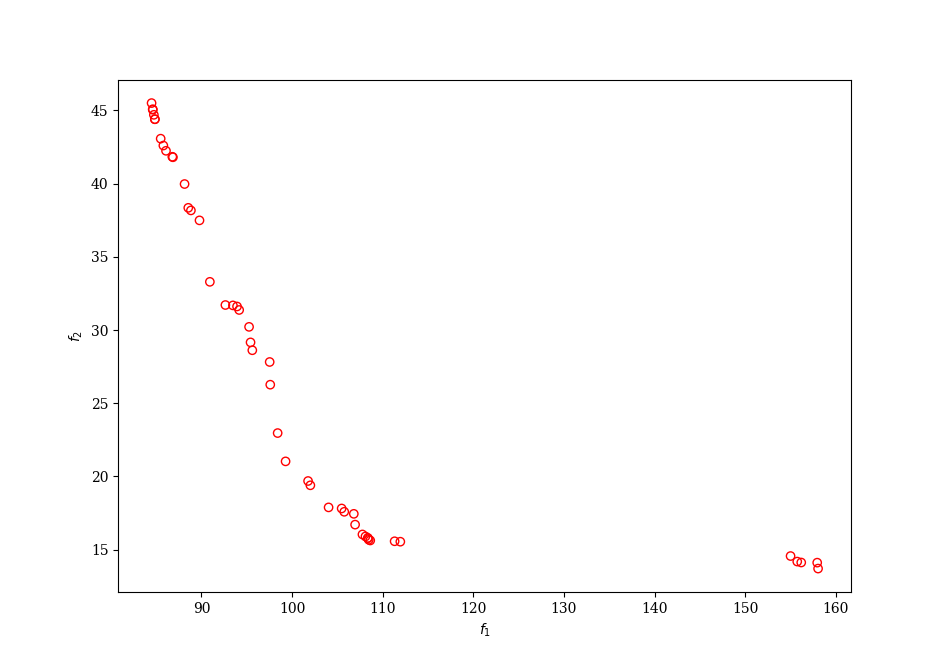
\includegraphics[width=.3\linewidth]{imatges/p2_l80.png}\hfill
  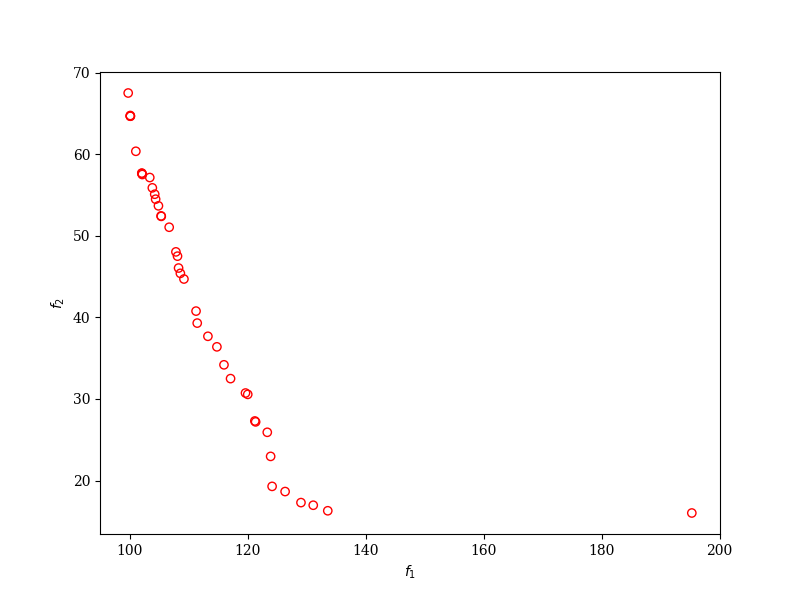
\includegraphics[width=.3\linewidth]{imatges/p2_l100.png}\hfill
  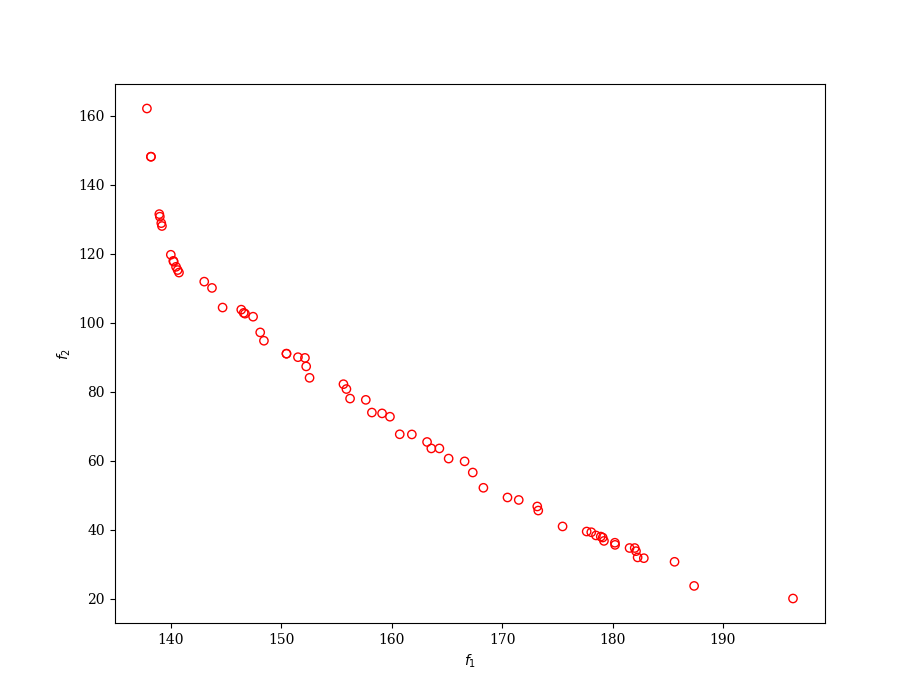
\includegraphics[width=.3\linewidth]{imatges/p2_l150.png}
  \caption{200 MW for distances, 80, 100 and 150 km respectively}
  \end{subfigure}\par\medskip
  \begin{subfigure}{\linewidth}
  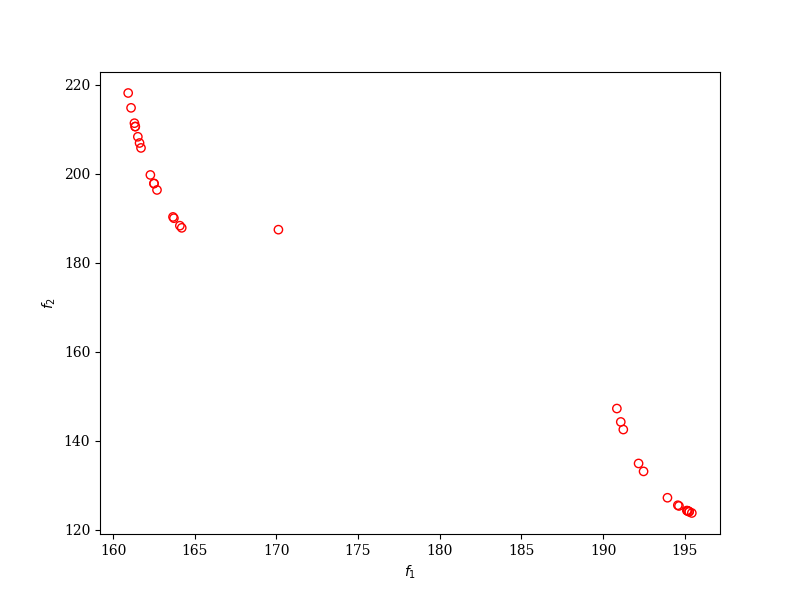
\includegraphics[width=.5\linewidth]{imatges/p10_l80.png}\hfill
  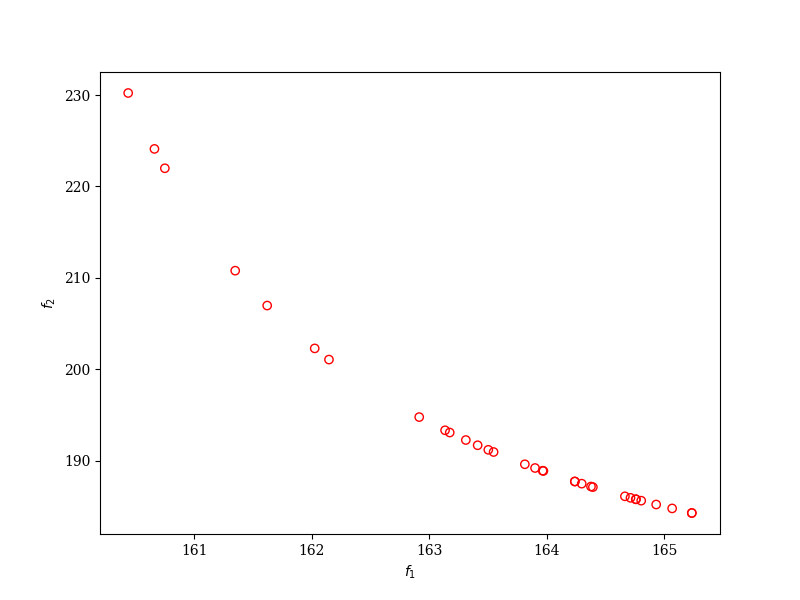
\includegraphics[width=.5\linewidth]{imatges/p10_l80_separating voltage.png}\hfill
  \caption{1000 MW for distance 80 km. It is clear the 2 sets represented by 2 or 3 cables in parallel. On the right, zoom to 2 cable zone}
  \end{subfigure}\par\medskip
\end{figure}

We also can see how it compares to a set of random evaluations:
\\
As we can see in this 200 MW case, the algorithm is able to find the pareto front 
positioned on the lower part of the plot, which is the optimal one. Note that for this case,
the upper set corresponds to 3 cables, that for small power plants lead to overvoltages, increasing
technical costs.

\begin{figure}[h]
  \begin{subfigure}{\linewidth}
  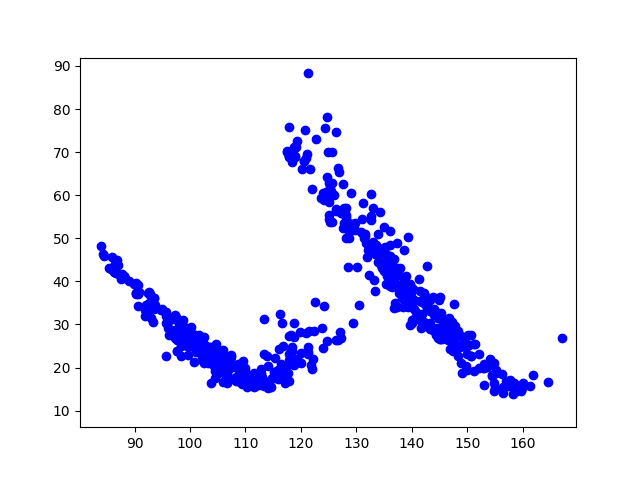
\includegraphics[width=.3\linewidth]{imatges/random_p2l80.png}\hfill
  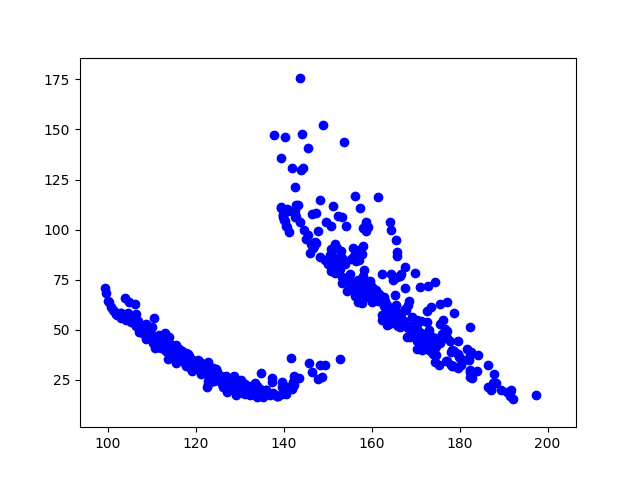
\includegraphics[width=.3\linewidth]{imatges/random_p2l100.png}\hfill
  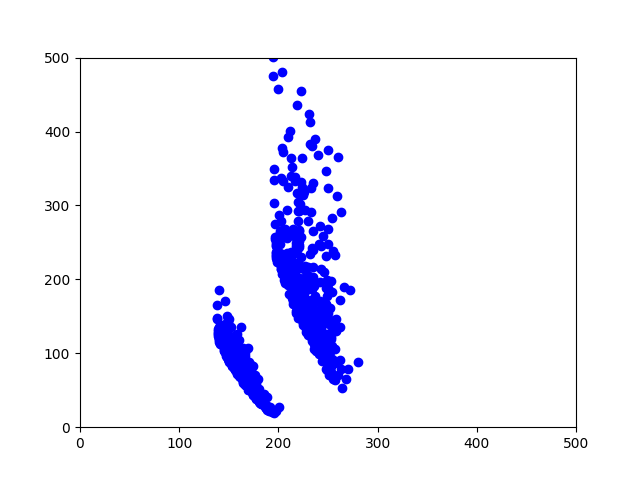
\includegraphics[width=.3\linewidth]{imatges/random_p2l150.png}
  \caption{200 MW for distances, 80, 100 and 150 km respectively with random evaluations}
  \end{subfigure}\par\medskip
  
\end{figure}
Another intersting insight from the random evaluations is that our exploration space seems to
be formed by n ( where n is the number of cable we are testing) convex sets.
\\
\\
Now we have to se how we select the optimal point in the pareto front. We can use the utopia point method,
which is a way to select the point that is closest to the anchor point in the pareto front. This is done
by normalizing the objectives and then selecting the point that minimizes the euclidean distance to the anchor point
in the normalized space.\\

\begin{figure}[h]
  \centering
  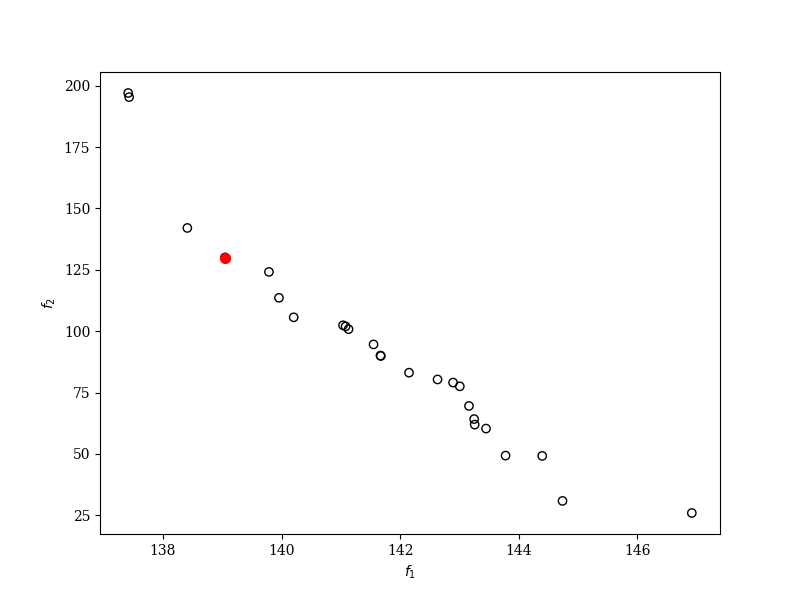
\includegraphics[width=.5\linewidth]{imatges/decision_opt_weight.png}
  \caption{Utopia point approach result (red dot) with equal weights for both objectives for 200 MW and 150 km}
  
\end{figure}

Ara cal mirar quis es el nostres set unknows solucio i comprar amb resultats paper. Aclarir que passa amb la compensacio que en alguns
casos mai la posa, fare ultima revisio funcions de costos i pw.
  
\end{document}
